% !TeX document-id = {b5392a94-51a3-49d1-9ba5-698bc09f9d35}
% !TeX encoding = UTF-8
% !TeX spellcheck = en_US
% !TeX TS-program = pdflatex
% !TeX TXS-program:bibliography = biber -l zh__pinyin --output-safechars %

%%%%%%%%%%%%%%%%%%%%%%%%%%%%%%%%%%%%%%%%%%%%%%%%%%%%%%%%
%%%% NOTE %%%%%%%%%%%%%%%%%%%%%%%%%%%%%%%%%%%%%%%%%%%%%%
%%%%%%%%%%%%%%%%%%%%%%%%%%%%%%%%%%%%%%%%%%%%%%%%%%%%%%%%
%
% Please do not touch the file `preamble.tex`
% ... which is auto-generated,
% ... and your changes might be OVERWRITTEN
% ... in later builds.
%
% Feel free to modify this file
% ... in any way you want!
%
% Bryan
%
%%%%%%%%%%%%%%%%%%%%%%%%%%%%%%%%%%%%%%%%%%%%%%%%%%%%%%%%
%%%% END of NOTE %%%%%%%%%%%%%%%%%%%%%%%%%%%%%%%%%%%%%%%
%%%%%%%%%%%%%%%%%%%%%%%%%%%%%%%%%%%%%%%%%%%%%%%%%%%%%%%%

\documentclass[a4paper
	,10pt
%	,twoside
]{article}

% to be `\input` in subfolders,
% ... therefore the path should be relative to subfolders.

\usepackage{iftex}
\ifPDFTeX
\else
	\usepackage[UTF8
		,heading=false
		,scheme=plain % English Document
	]{ctex}
\fi
%\ctexset{autoindent=true}
\usepackage{indentfirst}

\input{../.modules/basics/macros.tex}
\input{../.modules/preamble_base.tex}
\input{../.modules/preamble_beamer.tex}
\input{../.modules/basics/biblatex.tex}


%Misc
	\usepackage{lilyglyphs}
	\newcommand{\indicator}{$\text{\clefG}$}
	\newcommand{\indicatorInline}{$\text{\clefGInline}$}

\newcommand{\legacyReference}{{
%	\clearpage\par
%	\quad\clearpage
	\def{\midquote}{\textbf{PAST WORK, AS TEMPLATE}}
	\newparagraph
}}

% Settings
\counterwithout{equation}{section}
\mathtoolsset{showonlyrefs=false}
%\DeclareTextFontCommand{\textbf}{\sffamily}

% Spacing
\geometry{footnotesep=2\baselineskip} % pre footnote split
\setlength{\parskip}{.5\baselineskip}
\renewcommand{\baselinestretch}{1.15}


%% List
%	\setlist*{
%		listparindent=\parindent
%		,labelindent=\parindent
%		,parsep=\parskip
%		,itemsep=1.2\parskip
%	}


\addtobeamertemplate{navigation symbols}{}{%
    \usebeamerfont{footline}%
%    \usebeamercolor[fg]{footline}%
    \hspace{1em}%
    \large\insertframenumber/\inserttotalframenumber
}

\makeatletter
\setbeamertemplate{headline}
{%
    \begin{beamercolorbox}[wd=\paperwidth,colsep=1.5pt]{upper separation line head}
    \end{beamercolorbox}
    \begin{beamercolorbox}[wd=\paperwidth,ht=2.5ex,dp=1.125ex,%
      leftskip=.3cm,rightskip=.3cm plus1fil]{title in head/foot}
      \usebeamerfont{title in head/foot}\insertshorttitle
    \end{beamercolorbox}
    \begin{beamercolorbox}[wd=\paperwidth,ht=2.5ex,dp=1.125ex,%
      leftskip=.3cm,rightskip=.3cm plus1fil]{section in head/foot}
      \usebeamerfont{section in head/foot}%
      \ifbeamer@tree@showhooks
        \setbox\beamer@tempbox=\hbox{\insertsectionhead}%
        \ifdim\wd\beamer@tempbox>1pt%
          \hskip2pt\raise1.9pt\hbox{\vrule width0.4pt height1.875ex\vrule width 5pt height0.4pt}%
          \hskip1pt%
        \fi%
      \else%  
        \hskip6pt%
      \fi%
      \insertsectionhead
    \end{beamercolorbox}
% Code for subsections removed here
}
\makeatother

\title{Understanding Supersymmetry}
\author{The Superfilm Club, Summer 2021 @ \textkai{近春园}}
\addbibresource{susy.bib}

\makeatletter
\newcommand{\nobeginpar}{\@beginparpenalty=10000}
\makeatother

\newcommand{\speaker}[1]{\noindent\textbf{Speaker:} #1}
\newcommand{\references}[1]{\noindent\textbf{References:} #1}

\let\narrowbar\bar
\newcommand{\thinbar}[1]{\narrowbar{#1}}
\renewcommand{\bar}[1]{\narrowbar{#1}}

\let\widebar\overline
\newcommand{\wbar}[1]{\widebar{#1}}

\def\vev#1{\ave{#1}}

\usepackage{pifont}
\newcommand{\quabla}{\text{\ding{113}\hspace{.1em}}}

\begin{document}
\maketitle
\pagenumbering{arabic}

%\vspace*{-.5\baselineskip}

This is a note for our recreational journal club on supersymmetry (SUSY). It is not meant to be self-contained; rather it's aimed to be an outline and a supplement for the main references listed below. We try not to repeat the main references too much, but to document our new understandings and additional references on relevant subjects. 

\setlength{\parskip}{.1\baselineskip}
\tableofcontents
\setlength{\parskip}{\parskipnorm}

%\pagebreak\thispagestyle{headless}
\addtocounter{section}{-1}
\section{Main References}
\raggedright
\begin{itemize}
\item Primary:
	\begin{itemize}[itemsep=\parskip]%[leftmargin=2em]
	\item[\cite{Argyres:1996abc}]\fullcite{Argyres:1996abc}
		\par \textit{Recommended by Yanyan.}
	
	\item[\cite{Figueroa-OFarrill:2001xbd}]\fullcite{Figueroa-OFarrill:2001xbd}
		\par \textit{Recommended by Mauricio.}
	
	\item[\cite{Hori:2003ic}]\fullcite{Hori:2003ic}
	
	\item[\cite{Freedman:2012zz}]\fullcite{Freedman:2012zz}
	
	\end{itemize}
\pagebreak[3]
\item Secondary:
	\begin{itemize}
	
	\item[\cite{Wess:1992cp}]\fullcite{Wess:1992cp}
	
	\item[\cite{figueroa2015majorana}]\fullcite{figueroa2015majorana}
	
	\item[\cite{VanProeyen:1999ni}]\fullcite{VanProeyen:1999ni}
		\par \textit{Recommended by Mauricio.}
	
	\item[\cite{Tachikawa:2018sae}]\fullcite{Tachikawa:2018sae}
		\par \textit{Recommended by Chi-Ming.}
	
	\item[\cite{Zhou:2018abc}]\fullcite{Zhou:2018abc}
	
	\item[\cite{Kapranov:2015nft}]\fullcite{Kapranov:2015nft}
		\par \textit{Recommended by Yuan.}
	
	\end{itemize}
\end{itemize}
\justifying

\pagebreak\thispagestyle{headless}
\section{Algebra \& Unitary Representations}
	\speaker{Yanyan ``Handsome'' Li}\\
	\references{
	\begin{enumerate}[noitemsep,topsep=0pt]
	\item \textcite{Argyres:1996abc}, \S5
	\item \textcite{Wess:1992cp}, Chapter II
	\end{enumerate}
	}\vspace{.5\baselineskip}
	
	The generic form of a 4D SUSY algebra with central charge is given by \cite{Wess:1992cp}:
	\begin{equation}
		\{ Q^i_\alpha, \bar{Q}_{\dot{\alpha},j} \}
		= 2\sigma^\mu_{\alpha\dot{\alpha}} P_\mu
			\delta^i_j,
	\quad
		\{ Q^i_\alpha, Q^j_{\beta} \}
		= 2\epsilon_{\alpha\beta} Z^{ij}
	\end{equation}
	Here $i,j$ labels $\mcal{N}$ ``flavors'' of SUSY. For minimal SUSY we have $\mcal{N} = 1$, and we can drop the $i,j$ indices. Also $Z^{ij} = -Z^{ji}$, so there is no central extension when $\mcal{N} = 1$. 
	
	$Q$ is understood as the ``square root'' of $P$. 
	Note that it's been a fine tradition\footnote{
		\textkai{优良传统}.
	} of physicists (and experimental mathematicians) to take the square root of un-rootable things. For example, $\sqrt{-1}$ gives us $i$, and $\sqrt{\Box^2} = \sqrt{-P_u P^\mu}$ gives us the $\gamma$ matrices (thanks to Dirac). On the other hand, the energy $P^0$ is now written as a sum of $\abs{Q}^2$, which guarantees its positivity. See \S9 of \textcite{Argyres:1996abc}. 
	
	\textit{Remarks:}
	\begin{enumerate}
	\item $Q$ carries a spinor index $\alpha$ (or $\dot{\alpha}$), so it lives in the spinor representation of the Lorentz group, or equivalently, the fundamental (spin-$\frac{1}{2}$) representation of the Spin group\footnote{
		See a surprisingly good summary of the topic on \wikiref{https://en.wikipedia.org/wiki/Representation\_theory\_of\_the\_Lorentz\_group\#Finite-dimensional\_representations}{Representation theory of the Lorentz group \# Finite-dimensional representations}. 
		
		Note that higher spin supercharges are not allowed, since they cannot combine into $P_\mu$ or $J_{\mu\nu}$, but they must, due to Coleman--Mandula. Moreover in 4D higher spin charges simply violate Haag--Łopuszański--Sohnius (the SUSY extension of Coleman--Mandula). A thorough introduction of this is given in \S32 of \textcite{Weinberg:2000cr}, Vol.\,III. 
		See also \https{physics.stackexchange.com/a/418025}. 
	}. 
	
	\item The structure of this algebra can be generalized to $D$ dimensions. In general, $Q$ transforms as a \mbox{(symplectic)}\footnote{
		Symplectic Majorana happens when the metric signature $p - q \equiv 3,4,5\,\mop{mod}\,8$. See e.g.~\textcite{figueroa2015majorana}, or \S3.3 and \S12.1 of \textit{Supergravity} \cite{Freedman:2012zz}, or Mauricio Romo's lecture notes. In Lorentzian signature ($p = D-1, q = 1$), this corresponds to $D = 5,6,7$ dimensions; see e.g.~Table B.1 of \textcite{Polchinski:1998rr}. A worked example in 6D is given by \cite{Gustavsson:2001uw}. 
		
		Also, higher form central charges are possible in higher dimensions. 
	} (pseudo)\footnote{
		Pseudo-Majorana spinors exist for spacetime signature $(p,q)$ if and only if Majorana spinors exist for $(q,p)$. See \textcite{figueroa2015majorana} and \S3.3 of \textit{Supergravity} \cite{Freedman:2012zz}. 
		
		From now on we will \textit{not} distinguish between pseudo-Majorana and Majorana spinors, as they are both ``real'' under \textit{charge conjugation}, which we will define in \S1.1. 
	} Majorana spinor. 
	
	\item Complex conjugation maps $Q_\alpha \mapsto \bar{Q}_{\dot{\alpha}}$. The supercharges have to live in a \textit{real} representation, where both $Q_\alpha$ and $\bar{Q}_{\dot{\alpha}}$ are included. Otherwise they can't combine into the Hermitian $P_\mu$. Here we've chosen to write the 4D charges as Weyl spinor $Q_\alpha$ with 2 complex components, but they are not actually Weyl; they are secretly Majorana with 4 real components. The translation between these two descriptions is documented in \S3.4.2 of \textit{Supergravity} \cite{Freedman:2012zz}. 
	
	\item $(Q_\alpha, \bar{Q}_{\dot{\alpha}})$ act like (fermionic) annihilation and creation operators (ladder operators). We can write down its unitary irreducible representations (unitary irreps) on the Hilbert space, following Wigner's little group representation for the Poincar\'e group. 
	\end{enumerate}
\subsection{More on conjugations}
	The bar in e.g.\ $\bar{Q}$ denotes \textit{some sort of} conjugation. In 4D it usually means Dirac or charge conjugation. 
	Dirac spinors exist in any dimension, but let's first look at \textit{even} dimensions, where a Dirac spinor can always be decomposed into 2 Weyl spinors:
	\begin{equation}
		\psi^\bullet
		= (\lambda^\alpha, \bar{\chi}_{\dot{\alpha}})
	\end{equation}
	This is because in even dimensions we have a chirality operator $\Gamma$ \cite{Polchinski:1998rr}: 
	\begin{equation}
		D = 2k + 2,
	\quad
		\Gamma = i^{-k} \Gamma^0 \cdots \Gamma^{D-1},
	\quad
		\Gamma^2 = 1,
	\quad
		\{\Gamma, \Gamma^\mu\} = 0
	\end{equation}
	$\Gamma$ is the generalization of $\gamma_5$ in 4D, and serves as a chirality operator that distinguishes the left and right handed part of a Dirac spinor. This gives us Weyl spinors with a definite chirality. We can then diagonalize $\Gamma$ such that it's all $+1$ on the upper half diagonal, and all $-1$ on the lower half diagonal. 
	
	There is no such chirality operator in odd dimensions, therefore in odd dimensions we don't have Weyl spinors at all, and there are only (symplectic) (pseudo) Majorana spinors. For example, in 5D $\gamma_5$ itself gets ``promoted'' to be the last $\gamma$ matrix\footnote{
		For more on this, see \S3.1.7 of \textit{Supergravity} \cite{Freedman:2012zz}. 
	}. 
	
	Back to even dimensions where $
		\psi^\bullet
		= (\lambda^\alpha, \bar{\chi}_{\dot{\alpha}})
	$, we have, up to various constant coefficients (which may depend on the dimension $D$),
	\begin{equation*}
	\small
	\newcommand{\coef}{\text{\tiny\#\,}}
	\renewcommand{\arraystretch}{1.2}
	\begin{array}{rccll}
	\textbf{Type of Conjugation}
		& \psi^\bullet 
		&=& (\lambda^\alpha,\bar{\chi}_{\dot{\alpha}})
%		\hspace*{.5em}
		& \textbf{Notes}\\
\midrule
	\text{Complex}
		& (\psi^*)^\bullet
		&\sim& (\bar{\lambda}^{\dot{\alpha}},\chi_{\alpha})
		& \text{Exchange $\alpha$ with $\dot{\alpha}$}
\\
	\text{Dirac}
		& (i\psi^\dagger\gamma_0)_\bullet
		&\sim& ({\chi}_\alpha,\bar{\lambda}^{\dot{\alpha}})
		& \text{Switch chirality (handedness)}
\\[.5ex]
	\text{Majorana}
		& (\psi\,\mcal{C})_\bullet = (\psi^\mrm{T} C)_\bullet
		&\sim& (\bar{\lambda}_{{\alpha}},{\chi}^{\dot{\alpha}})
			_{D\equiv 4},
		& \\
	&
		&\sim& ({\chi}_{\dot{\alpha}},\bar{\lambda}^{{\alpha}})
			_{D\equiv 2},
		\,\cdots
		& \text{Transpose (dual representation)}
\\[.5ex]
	\text{Charge}
		& (i\gamma_0\,C^{-1} \psi^*)^\bullet
		&\sim& ({\chi}^\alpha,\bar{\lambda}_{\dot{\alpha}})
			_{D\equiv 4},
		& \\
	&
		&\sim& (\bar{\lambda}^{\dot{\alpha}},{\chi}_\alpha)
			_{D\equiv 2},
		\,\cdots
		& [\text{Majorana}]^{-1} \circ [\text{Dirac}]
	\end{array}
	\end{equation*}
	Remarks:
	\begin{itemize}[beginpenalty=10000]
	
	\item In components, the bar notation is actually redundant. It simply indicates that we have taken some sort of conjugation \cite{Freedman:2012zz}. To know what kind of conjugation this is, we have to read the indices. 
	
		\begin{itemize}
		\item Dotted indices such as $\dot{\alpha}$ denote the complex conjugate representation. 
		
		\item The position of an index indicates how it transforms under the Spin group (covariant spinor or its dual). 
		\end{itemize}
	
	\item $C\id{^\bullet_\bullet}$ is the charge conjugation matrix, while $\mcal{C}_{\bullet\bullet}$ is the corresponding bilinear form. $\mcal{C}_{\bullet\bullet}$ works like a metric, and is used to raise and lower the spinor indices. It is anti-symmetric, compatible with the anti-commuting $\psi$. 
	
	\item $\mcal{C}$ is sensitive about the dimension $D$, and so is the Majorana conjugation. For example, in 4D $\mcal{C}$ is block diagonal, thus it does not switch $\lambda$ with $\chi$. In 2D, however, $\mcal{C}$ is basically the antisymmetric $\epsilon_{\alpha\dot{\alpha}}$, therefore it does switch $\lambda$ with $\chi$. 
	
	\item In 4D, charge conjugation is basically Dirac conjugation, but without the lowering of indices with $\mcal{C}$. We see that in 4D, when $\lambda = \chi$, $\psi$ is invariant under charge conjugation: $\psi^C = \psi$. This is the reality condition, and $\psi = (\chi^\alpha,\bar{\chi}_{\dot{\alpha}})$ is a \textit{Majorana spinor}. 
	
	In 2D, on the other hand, we see that Majorana conjugation is basically Dirac conjugation, but without the complex conjugation $\alpha \leftrightarrow \dot{\alpha}$. Therefore, charge conjugation is basically complex conjugation. The reality condition $\psi^C = \psi$ now reduces to $\lambda^* = \lambda$, $\chi^* = \chi$. This gives us 2 independent \textit{Majorana--Weyl} spinors. 
	
	\item Charge conjugation is convenient as it preserves the ordering of matrices (since it does not include a transpose). One can think of it as a physical replacement for the na\"ive complex conjugation. 
	
	\item When the indices are suppressed, matrices are assumed to be contracted with $\mcal{C}$. In this case we do need to specify the meaning of $\bar{\psi}$. 
	
	In 4D we usually take $\bar{\psi}$ to denote Dirac conjugate, as in \S2 of \textit{Supergravity} \cite{Freedman:2012zz}. However, since \S3 they switch their conventions and $\bar{\psi}$ denotes Majorana conjugate instead\footnote{
		See \S3.2 of \textcite{Freedman:2012zz}. 
	}. \textcite{Polchinski:1998rr} seems to consistently define $\bar{\psi}$ as Dirac conjugate\footnote{
		See (B.1.29) of \textcite{Polchinski:1998rr}, Vol.\,II. 
	}. 
	
	\end{itemize}
	
	\newparagraph
	These have always been confusing concepts for me. For a friendly introduction to Majorana spinors in 4D, check out \textcite{Pal:2010ih}. For a pedagogical treatment in general dimensions, see \S2 and \S3 of \textit{Supergravity} \cite{Freedman:2012zz}. One can then compare it to the results in 4D, discussed in Appendix A.4 to A.8 of \textcite{Figueroa-OFarrill:2001xbd}. See also \textcite{Tachikawa:2018sae}. Fortunately their conventions seem to agree with each other, for most of the time. 
	
\subsection{Equal amount of bosonic \& fermionic (excited) states}
	$Q$ maps bosonic states to fermionic states, and vice versa. We thus have:
	\begin{equation}
		(-1)^F Q = - Q\,(-1)^F
	\label{eq:fermion_number_sign}
	\end{equation}
	$F$ is the fermion number operator. $(-1)^F$ can be explicitly constructed from a $2\pi$ rotation \cite{Argyres:1996abc,Witten:1982df}: \mbox{$
		(-1)^F = e^{2\pi i J_z}
	$}. This follows from the fact that spin-$\frac{1}{2}$ objects gain a $(-1)$ factor under a $2\pi$ rotation. 
	
	On the other hand, recall that $Q$ acts as a ladder operator, therefore:
	\begin{equation}
		F Q = Q\,(F \pm 1),
	\quad\text{i.e.}\quad
		[F, Q] = \pm Q
	\label{eq:fermion_number_R_symmetry}
	\end{equation}
	The \mquote{+} sign corresponds to $\bar{Q}_{\dot{\alpha}}$, while the \mquote{-} sign corresponds to $Q_\alpha$. 
	\eqref{eq:fermion_number_sign} can thus be understood as the exponential of \eqref{eq:fermion_number_R_symmetry}, i.e.\ $(-1)^F = e^{i\pi F} = e^{-i\pi F}$,
	\begin{equation}
		(-1)^F Q\,(-1)^F
		= e^{i\pi F} Q\,e^{-i\pi F}
		= e^{\pm i\pi} Q
		= -Q
	\end{equation}
	
%\pagebreak[3]
	
	There is more story behind \eqref{eq:fermion_number_R_symmetry}; in fact, $F$ generates an automorphism of the SUSY algebra. It is part of the \textit{R-symmetry}, and can be added to the algebra as an extension. 
	In Lorentzian 4D, the maximal amount of R-symmetry is $\mrm{U}(\mcal{N})$, and $F$ is the generator of the central $\mrm{U}(1)$ subgroup:
	\begin{equation}
		\mrm{U}(\mcal{N})
		= \mrm{U}(1) \rtimes \mrm{SU}(\mcal{N})
	\end{equation}
	$\mrm{U}(\mcal{N})$ comes from the maximal extension of the SUSY algebra. It is common that, given a specific theory, only some of the R-symmetries are preserved, while others are broken. Even the fermion number $e^{i\theta F} \in \mrm{U}(1)$ can be broken, but it seems that the $\mbb{Z}_2$ subgroup generated by $e^{i\pi F} = (-1)^F$ always survives \needcites. 
	
	\newparagraph
	Using \eqref{eq:fermion_number_sign} along with a bit of algebra \cite{Wess:1992cp}, we find that:
	\begin{equation}
		0 = \Tr \pqty\Big{
			(-1)^F
			\{ Q^i_\alpha, \bar{Q}_{\dot{\alpha},j} \}
		}
		= 2\sigma^\mu_{\alpha\dot{\alpha}} \delta^i_j
			\Tr \pqty\Big{
			(-1)^F P_\mu
		}
	\end{equation}
	This implies that for fixed $P_\mu \ne 0$ we have:
	\begin{equation}
		\Tr_P (-1)^F = 0,
	\quad
		\mcal{H}_P = \Bqty\big{ \ket{P_\mu} }
	\end{equation}
	
	This means that we have equal amount of bosonic \& fermionic (excited) states at each energy level in a SUSY theory. 
	Note that for ground states $P_\mu = 0$, we don't necessary have $\Tr_0 (-1)^F = 0$. In fact, this is precisely the \textit{Witten index} \cite{Witten:1982df}:
	\begin{equation}
		\Tr\,(-1)^F e^{-\beta H}
	\end{equation}
	Here the trace goes over the entire Hilbert space, but only the zero energy ground states actually contribute, since excited states are all paired up and canceled. The $e^{-\beta H}$ factor can be understood as regularization, and the final answer should simply be $\Tr\,(-1)^F = \Tr_0 (-1)^F$ with no $\beta$ dependence. In fact, it's also robust under small deformations of the theory, i.e.\ it's a \textit{topological invariant} of the theory. 
	
	\begin{itemize}
	\item If one finds that $\Tr\,(-1)^F \ne 0$, that means there is at least one zero energy ground state, namely, SUSY is unbroken. 
	
	\item On the other hand, if SUSY is spontaneously broken, then there are no zero energy ground states, so $\Tr\,(-1)^F = 0 - 0 = 0$. 
	
	\item It's also possible to have $\Tr\,(-1)^F = 0$ while SUSY is unbroken, namely the ground states also pair up exactly: $N_B = N_F$. However, practically speaking, SUSY is broken, since if not, an arbitrarily small perturbation by a relevant operator will give energy to the ground state, thus breaking SUSY \cite{Argyres:1996abc}. 
	\end{itemize}
	
\subsection{Witten index \& elliptic genus}
	
	The Witten index can actually be understood as the index of an operator \cite{Witten:1982df}. We may split the Hilbert space $\mcal{H}$ of our theory into bosonic and fermionic subspaces:
	\begin{equation}
		\mcal{H} = \mcal{H}_B \oplus \mcal{H}_F,
	\end{equation}
	\vspace*{-\baselineskip}
	\begin{equation}
		Q(\mcal{H}_B) \equiv \mcal{Q(}\mcal{H}_F),
	\quad
		Q(\mcal{H}_F) \equiv \mcal{Q}^\dagger(\mcal{H}_B),
	\end{equation}
	Here we've used the self-adjoint Majorana super charge $Q$, which decomposes into:
	\begin{equation}
		\mcal{Q}\colon \mcal{H}_B \longto \mcal{H}_F,
	\quad
		\mcal{Q}^\dagger\colon \mcal{H}_F \longto \mcal{H}_B,
	\end{equation}
	
	Zero energy bosonic states are zero-modes of $M$, while zero energy fermionic states are zero-modes of $M^\dagger$. We see that the Witten index is precisely the index of $M$:
	\begin{equation}
		\Tr\,(-1)^F
		= N_B - N_F
		= \dim \ker \mcal{Q} - \dim \ker \mcal{Q}^\dagger
	\end{equation}
	For more on this, check out the first few sections of the original paper: \textcite{Witten:1982df}. 
	
	\newparagraph
	A more refined invariant in 2D that involves only the left-moving (or right-moving) part of theory is the \textit{elliptic genus}. For 2D $\mcal{N} = (2,2)$ superconformal theory (SCFT), the fermion number:
	\begin{equation}
		F = F_V = J_0 + \bar{J}_0
	\end{equation}
	Here $J(z),\bar{J}(\bar{z})$ are bosonic currents. They can be understood as the infinite dimensional enhancement of the R-symmetry generators in an SCFT, while their 0-modes $J_0,\bar{J}_0$ corresponds to the original R-symmetry generators in the SUSY algebra. $F_V = J_0 + \bar{J}_0$ is the $\mrm{U}(1)_V$ generator, while $F_A = \bar{J}_0 - J_0$ is the $\mrm{U}(1)_A$ generator. 
	The \mbox{subscript V} stands for ``vector'', meaning that the supercharge $Q^i$ transforms as a vector with index $i$ under the $\mrm{U}(1)_V$ action: all components labeled by $i$ gains the same phase shift under $\mrm{U}(1)$. The \mbox{subscript A} stands for ``axial'', meaning that $Q^i$ transforms in an axial representation of $\mrm{U}(1)$, where the group action discriminates between left and right-handed components\footnote{
		This might generate some confusions when compared to 4D: if we think of $Q,\bar{Q}$ as two components of a Majorana spinor (in the Weyl basis), then the fermion number $\mrm{U}(1)$ looks like an \textit{axial} symmetry, as is given in \eqref{eq:fermion_number_R_symmetry}. This is indeed the case in 4D, where charge conjugation switches $Q$ and $\bar{Q}$, as described in \S1.1. We will come back to this in \S\ref{subsect:anomaly}, where we discuss axial anomaly. 
		
		However, charge conjugation in 2D looks very different: it actually switches between $Q_+$ and $Q_-$, where $\mquote{\pm}$ is the $\mcal{N} = 2$ indices. This is consistent with our discussions in \S1.1. 
		For example, a chiral $(2,0)$ theory is constructed not by throwing away $\bar{Q}$, but by throwing away $Q_-$ and $\bar{Q}_-$; see \S12.5.2 of \textit{Mirror Symmetry} \cite{Hori:2003ic}. 
	}. 
	
	We can now define the elliptic genus, which looks just like the Witten index but with an additional insertion $y^{J_0}$, while the trace is restricted to the R-R sector:
	\begin{equation}
		\mrm{EG}(\tau,z)
		= \Tr_{\text{R-R}} \pqty{
			(-1)^{J_0 + \bar{J}_0}
			y^{J_0}
			q^{L_0 - \frac{c}{24}}
			\bar{q}^{\bar{L}_0 - \frac{c}{24}}
		}, \quad y = e^{2\pi i z}
	\end{equation}
	Here R-R stands for Ramond-Ramond, i.e.\ left and right-moving states both with periodic boundary conditions along the spatial cycle\footnote{
		In the path integral formalism, the thermal circle is also periodic due to the $(-1)^F$ insertion. 
	}. 
	For a review on this, see e.g.~\cite{Anagiannis:2018jqf}. 
	
	$z$ is understood as the chemical potential associated with the charge $J_0$. Note that there is no $\bar{\tau}$ dependence in EG, for the same resaon that there is no $\beta$ dependence in the Witten index. Also the elliptic genus gets reduced to the Witten index when we take $z = 0$, and in this case the $\tau,\bar{\tau}$ dependences all drop out; here we note that although we often trace over the entire R-R sector for the Witten index, only the supersymmetric R-R ground states actually contributes. 
	
	On the other hand, for general $z$ the elliptic genus counts states that are R ground state on the one side, but includes R excited states on the other side. 
	It contains a lot more information but still has the rigidity property of the Witten index which makes it possible to compute for many SCFTs, and as such it offers a good balance between information content and computability. 
	
	Geometrically, the elliptic genus is a generalization of the usual genus. In particular, for $z = 0$ we recover the Witten index, which evalutates to the Euler characteristic $\chi(M)$, where $M$ is the \textit{target} manifold\footnote{
		See Chapter 10.4 of \textit{Mirror Symmetry} \cite{Hori:2003ic}, or \textcite{Witten:1982df}. See also \cite{MauricioStuff} and:
		\begin{itemize}[
%			topsep=0ex,
			noitemsep,
			leftmargin=3em
		]
		\item \https{physicsoverflow.org/23261}
		\item \https{physics.stackexchange.com/a/183620}
		\end{itemize}
%		\vspace{-.8\baselineskip}
	}. This is due to the fact that $Q$ gets identified with the de Rham differential $\mquote{\dd}$ on the target $M$. This should become apparent as we introduce the superfield formalism and K\"ahler geometry in \S2. 
	
\subsection{Representations of the SUSY algebra}
	We've noted that $(Q_\alpha, \bar{Q}_{\dot{\alpha}})$ act like ladder operators, therefore we can construct a highest weight representation starting from some \textit{Clifford vacuum} $\ket{\Omega}$ that is annihilated by $Q_\alpha,\alpha = 1,2$, and also $J_z$, which is the angular momentum along the $z$ direction. 
	
	Note that $\ket{\Omega}$ is only a highest weight state in a representation of the $\{Q,Q\}$ subalgebra, defined in the \textit{comoving frame} of a particle; it is not the Poincar\'e invariant vacuum $\ket{0}$ that we usually talk about in QFT. 
	
	For 4D $\mcal{N} = 1$, suppose $\ket{\Omega}$ has spin $j$, namely $J_z \ket{\Omega} = j\ket{\Omega}$, then we have:
	\begin{itemize}[leftmargin=0pt,itemindent=*]
	\item \textbf{Massive representation:}
		\begin{equation}
			\ket{\Omega},
			\ \bar{Q}_{\dot{\alpha}=1,2}
				\ket{\Omega},
			\ \bar{Q}_{\dot{1}}\bar{Q}_{\dot{2}}
				\ket{\Omega}
		\end{equation}
		i.e.~a $1+2+1 = 4$ dimensional representation of the $\{Q,Q\}$ subalgebra. 
		Note that this is \textit{not} yet invariant under the little group $\mrm{Spin}(3) \supset \mrm{SO}(3)$. For that we need to include the $\mrm{Spin}(3)$ descendents by acting on the angular momentum lowering operator $J_-$. 
	\end{itemize}
	
	Before actually doing that, let's first look at the spin of these states. 
	The $J_z$ eigenvalue for these states can be read out from the $[J_z,\bar{Q}_{\dot{\alpha}}]$ commutator. Recall that $\bar{Q}_{\dot{\alpha}}$ itself carries a spinor index $\dot{\alpha}$, namely it also lives in a representation of the Lorentz group! 
	The result is that\footnote{
		See Mauricio Romo's lecture notes, and also \cite{Terning:2006bq}. 
	} $\bar{Q}_{\dot{\alpha}=1,2} \ket{\Omega}$ will be a $\mrm{Spin}(3)$ highest weight state of $J_z$ eigenvalue $j \pm \frac{1}{2}$,
	\begin{equation}
		J_z\,\pqty\Big{
			\idty,
			\ \bar{Q}_{\dot{\alpha}=1,2},
			\ \bar{Q}_{\dot{1}}\bar{Q}_{\dot{2}}
		} \ket{\Omega} = \pqty\Big{
			j,\ j\pm\tfrac{1}{2},\ j
		} \ket{\Omega}
	\end{equation}
	
	\begin{itemize}[label=--]
	\item \textbf{Chiral multiplet} $\{\phi,\psi_\alpha\}$: for $j = 0$, the $\pm\frac{1}{2}$ states actually combine to live in a \textit{single} $\mrm{Spin}(3)$ fundamental representation, denoted as $\frac{1}{2}$. 
	In terms of field content, we have 1 Weyl spinor $\psi_\alpha$ and 2 real scalars $\phi_{1,2}$, which can be combined into 1 complex scalar $\phi$. These are ``quarks'' and ``squarks''. 
	
	\item \textbf{Vector multiplet} $
		\{\phi',\psi_\alpha,\lambda_\alpha,A'_\mu\}
	$: for $j = \frac{1}{2}$, the $j\pm\frac{1}{2} = 0,1$ states and their $\mrm{Spin}(3)$ descendants live in a $0\oplus 1$ representation of $\mrm{Spin}(3)$. 
	In terms of field content, we have 1 \textit{real} scalars $\phi'$, 1 massive vector $A'_\mu$, and 2 Weyl spinors $\psi_\alpha, \lambda_\alpha$. 
	\end{itemize}
	
	In general, the $j \pm \frac{1}{2}$ states and their $\mrm{Spin}(3)$ descendants live in a $
		\pqty{j - \frac{1}{2}}
		\oplus
		\pqty{j + \frac{1}{2}}
	$ representation of $\mrm{Spin}(3)$. We can check that the degrees of freedom indeed match:
	\begin{equation}
	\begin{array}{ccccc}
		\Bqty\Big{
			(J_-)^k\,
			\bar{Q}_{\dot{\alpha}=1,2}
			\ket{\Omega}
		}_{k\,\le\,2j+1}
		&=& \pqty{j - \tfrac{1}{2}}
			&\oplus&
			\pqty{j + \tfrac{1}{2}}
	\\[2ex]
		2\times (2j+1)
		&=& 2\,(j-\tfrac{1}{2}) + 1
			&+&
			2\,(j+\tfrac{1}{2}) + 1
	\end{array}
	\end{equation}
	Here $J_-$ is the $\mrm{Spin}(3)$ lowering operator. 
	Namely, including the $\mrm{Spin}(3)$ descendants, the dimension of the $\mrm{super} \times \mrm{Spin}(3)$ representation is thus $4\times (2j+1)$. 
	Note that for $j = 0$ the situation is special; in that case we simply have:
	\begin{equation}
	\begin{array}{ccccc}
		\Bqty\Big{
			\bar{Q}_{\dot{1}} \ket{\Omega},
			\ \bar{Q}_{\dot{2}} \ket{\Omega}
			\propto J_-\,
				\bar{Q}_{\dot{1}} \ket{\Omega}
		} 
		&=& \pqty{\tfrac{1}{2}}
	\\[2ex]
		2\times (2\times 0+1)
		&=& 2\,(\tfrac{1}{2}) + 1
	\end{array}
	\end{equation}
	
	\begin{itemize}[leftmargin=0pt,itemindent=*]
	\item \textbf{Massless representation:}
		\begin{equation}
			\ket{\Omega},
			\ \bar{Q}_{\dot{\alpha}=1} \ket{\Omega}
		\end{equation}
		i.e.~a $1+1 = 2$ dimensional representation of the $\{Q,Q\}$ subalgebra. They have helicity $\lambda,\lambda + \frac{1}{2}$. Combined with their CPT conjugates, we have 4 states with helicity: $\pm\lambda,\pm\pqty{\lambda + \frac{1}{2}}$. 
	\end{itemize}
	
	\begin{itemize}[label=--]
	\item \textbf{Chiral multiplet} $\{\phi, \psi_\alpha\}$: for $\lambda = 0$, we have 2 real scalars $\phi_{1,2}$ (or 1 complex scalar $\phi$) and 1 Weyl spinor $\psi_\alpha$. Note that the field content is precisely the same as the massive chiral multiplet. 
	
	\item \textbf{Vector multiplet} $\{\lambda_\alpha, A_\mu\}$: for $\lambda = \frac{1}{2}$, we have 1 massless vector $A_\mu$ and 1 Weyl spinor $\lambda_\alpha$. These are gauge bosons and ``gauginos''. Note that this multiplet is significantly ``smaller'' than the massive vector multiplet. 
	\end{itemize}
	
	Starting with higher spin Clifford vacua results in multiplets with spins higher than 1. This is undesirable for \textit{massless} particles in non-gravitational theories, due to \textit{Weinberg--Witten}\footnote{
		See e.g.\ \https{physics.stackexchange.com/a/15164}. 
	}. 
	
	Also, the multiplets grow large if we have extended SUSY, and the massless representation contains states with helicity $\lambda,\cdots,\lambda + \frac{\mcal{N}}{2}$ \cite{Terning:2006bq}. 
	
	\begin{itemize}
	\item \textbf{16 supercharges without gravity:} $\abs{\lambda} \le 1$, $\abs{\lambda + \frac{\mcal{N}}{2}} \le 1$, which give us $\mcal{N} = 4$ in 4D. There are in total 16 supercharges: $
		\{ Q^i_\alpha, \bar{Q}_{\dot{\alpha},j} \}_{i,j = 1,\cdots 4}
	$. In fact 16 is the maximal amount of SUSY in \textit{any} dimension, if we want spin $\le 1$. 
	
	\item \textbf{32 supercharges with gravity:} $\abs{\lambda} \le 2$, $\abs{\lambda + \frac{\mcal{N}}{2}} \le 2$, which give us $\mcal{N} = 8$ supergravity (SUGRA) in 4D. Similarly 32 is the maximal amount of SUSY in any dimension, if we want spin $\le 2$. For example, in 11D $\mcal{N} = 1$ we have precisely 32 supercharges, and the SUGRA multiplet is the smallest multiplet. Therefore the maximum dimension for SUGRA is 11. 
	\end{itemize}
	Note that these massless supermultiplets have helicity $-\abs{\lambda},\cdots,\abs{\lambda}$ and is thus CPT self-conjugate. 
	
	\newparagraph
	We actually care more about the massless representations and less about the massive ones. The reason is that massless representations are considered more ``fundamental'', since masses are usually generated dynamically through spontaneous symmetry breaking. This philosophy is discussed in later sections in more details. 
	
	For 4D $\mcal{N} = 1$, we can already see this by counting degrees of freedom:
	\begin{equation}
	\begin{array}{ccccc}
		\text{(massless chiral)}
		&\oplus&
		\text{(massless vector)}
		&\cong&
		\text{(massive vector)}
	\\[1ex]
		\{\phi, \psi_\alpha\}
		&\oplus&
		\{\lambda_\alpha, A_\mu\}
		&\cong&
		\{\phi',\psi_\alpha,\lambda_\alpha,A'_\mu\}
	\end{array}
	\end{equation}
	This is indeed the case dynamically: massive vector multiplets arise by a supersymmetric analog of the Higgs mechanism \cite{Argyres:1996abc}.
	$\phi$ is like the complex Higgs field. One component (the Goldstone mode) of $\phi$ gets ``eaten'' by the gauge field $A_\mu$ through symmetry breaking. The degrees of freedom combine into the massive vector $A'_\mu$. The other component of $\phi$ remains as the real scalar $\phi'$. 
	
\section{Superspace \& Superfields}
	\speaker{Ban ``Bo'' Lin}\\
	\references{
	\begin{enumerate}[noitemsep,topsep=0pt,beginpenalty=10000]
	\item \textcite{Argyres:1996abc}, \S6 \& \S9
	\item \citetitle{Hori:2003ic} \cite{Hori:2003ic}, Chapter 12
	\end{enumerate}
	}\vspace{.5\baselineskip}
	
	Superspace \& superfields encode the SUSY transformation implicitly, so we can write down manifestly SUSY-invariant actions. This is exactly similar to how we write down diff-invariant actions in usual QFT.
	
	A generic superfield will give a \textit{reducible} representation of the superalgebra. To get an \textit{irreducible} representation (\textit{irrep}), we must impose a constraint on the superfield which (anti-)commutes with the superalgebra. There are two possibilities for 4D $\mcal{N} = 1$:
	\begin{enumerate}%[noitemsep]
	\item \textbf{Reality condition:} $\bar{V} = V$, this gives us the vector superfield; see \S10.1 of \textcite{Argyres:1996abc}. We shall revisit this in \S6. For now we will proceed to the next condition, which is:
	
	\item \textbf{Chirality condition:}
	\begin{equation}
		\bar{D}_{\dot{\alpha}} \Phi = 0
	\quad\Leftrightarrow\quad
		\Phi = \Phi(y,\theta),
	\quad
		y^\mu \equiv x^\mu
			+ i\theta \sigma^\mu \bar{\theta}
	\end{equation}
	This gives us the chiral superfield $\Phi$. It can be expanded in components as follows:
	\begin{equation}
	\begin{aligned}
		\Phi
		&= \phi(y) + \sqrt{2}\,\theta\,\psi(y)
			+ \theta^2 F(y) \\
		&= \phi(x) + \cdots
			+ \theta^2 F(x)
	\end{aligned}
	\label{eq:chiral_components}
	\end{equation}
	Note that the first line is not the end of the story; to get to the actual component fields we have to write everything in terms of $(x,\theta)$, like in the second line. 
	\end{enumerate}
	
	For 4D $\mcal{N} = 1$, a generic SUSY-invariant Lagrangian of the chiral superfields $\Phi$ is given by:
	\begin{equation}
		\mcal{L}
		= \int \dd[4]{\theta} \mcal{K}(\Phi, \bar{\Phi})
			+ \int \dd[2]{\theta}
				\mcal{W}(\Phi)
			+ \int \dd[2]{\bar{\theta}}
				\wbar{\mcal{W}}(\bar{\Phi})
	\end{equation}
	$\Phi$ can be a collection of chiral superfields $\Phi^a$, but here for simplicity we've dropped the $a$ indices.
	
	\begin{enumerate}
	\item $\mcal{K}(\Phi, \bar{\Phi})$ is the \textbf{K\"ahler potential} and gives us the kinetic terms of the component fields. 
	The target automatically becomes a K\"ahler manifold where the component field $\phi$ is the target coordinate. A non-degenerate kinetic term corresponds to a positive definite metric \cite{Hori:2003ic}:
	\begin{equation}
		g_{i\wbar{j}}
		= \pdd{i} \pdd{\wbar{j}}
			\mcal{K}(\Phi, \bar{\Phi}),
	\quad \pdd{i} = \pdv{\phi^i}
	\end{equation}
	On the other hand, the fermion fields $\psi$ are naturally interpreted as vectors in the tangent space to the K\"ahler manifold:
	\begin{equation}
		\psi, \bar{\psi}
		\in \Gamma\pqty{
				\Sigma,
				\phi^* \mrm{T}M \otimes \mbb{C}
			}
	\end{equation}
	Here $\Gamma\pqty{\Sigma,-}$ stands for sections of some bundle over $\Sigma$. See e.g.~\textit{Mirror Symmetry} \cite{Hori:2003ic}. 
	
%	\pagebreak[3]
	
	\item $\mcal{W}(\Phi)$ is the \textbf{superpotential;} it is holomorphic w.r.t.\,$\Phi$, and it generates the potential and interaction vertices for the component fields. It's also called an \textbf{$F$-term}, probably due to the fact that:
	\begin{equation}
		\text{For}\ \,\mcal{W} = \Phi,
	\ \,
		\int \dd[2]{\theta} \mcal{W}
		= F(x)
	\end{equation}
	Here $F(x)$ is the last component of a chiral superfield \eqref{eq:chiral_components}. Generally, we have:
	\begin{equation}
		\int \dd[2]{\theta}
			\mcal{W}(\Phi^i)
		= F^i \pdd{i}\mcal{W}
			- \frac{1}{2} \psi^i \psi^j
				\pdd{i} \pdd{j} \mcal{W}
	\end{equation}
	
	\end{enumerate}
	
\subsection{$F$-term and the classical vacua}
	A full expansion of the Lagrangian $\mcal{L}$ (including $\mcal{K}$ and $\mcal{W}$) reveals that $F$ has no kinetic term and is quadratic in the action, thus it can be safely integrated out. The equation of motion is simply:
	\begin{equation}
		F^i = - g^{i\wbar{i}}
			\pdd{\wbar{i}} \wbar{\mcal{W}}
		+ \frac{1}{2}\,\Gamma^i_{jk} \psi^j \psi^k
	\end{equation}
	This gives a potential for the scalar component $\phi$:
	\begin{equation}
		V(\phi,\bar{\phi})
		= \norm{\pd\mcal{W}}^2
		= g^{i\wbar{j}}
			\,\pdd{i} \mcal{W}
			\,\pdd{\wbar{j}} \wbar{\mcal{W}}
		\xlongequal{\vev{\psi \psi} = 0}
		g_{i\wbar{j}} F^i \wbar{F}^{\wbar{j}}
		= \norm{F}^2
	\end{equation}
	Here we've used the fact that $\vev{\psi \psi} = 0$, so only the $\pd\mcal{W}$ term contributes to the VEV $\vev{F}$. Note that the non-zero fermion propagator is given by $\vev{\psi \bar{\psi}}$ instead. 
	
	The classical vacua satisfy $\pd_i V = 0$. 
%	Spontaneous breaking of internal symmetry happens if we have $\vev{\phi} \ne 0$. 
	On the other hand, we see that $V\ge 0$ for a positive-definite metric $g_{i\wbar{j}}$, therefore if $V = 0$ we have $\pdd{i} V = 0$ and $\pdd{i} \mcal{W} = 0$. In this case we have SUSY vacua, i.e.~SUSY is unbroken. 
	
	In summary,
	\begin{itemize}[noitemsep]
	\item Vacua: $
		\pdd{i} V
		= \pdd{i}\,\pqty\big{\norm{\pdd{i} \mcal{W}}^2}
		= 0
	$
	\item SUSY vacua: $\pdd{i} \mcal{W} = 0$, which implies $V = 0$ thus $\pdd{i} V = 0$. 
	\end{itemize}
	Spontaneous breaking of SUSY happens if $\pdd{i} V = 0$ while $V \ne 0$, namely we don't have a SUSY vacua. Fig.\,1.4 of \textcite{Terning:2006bq} is a nice summary of the situations. These backgrounds will come in handy in later sections. 
	
\section{Holomorphy and Non-renormalization}
	\speaker{Wen-Xin ``Bryan'' Lai}\\
	\references{
	\begin{enumerate}[noitemsep,topsep=0pt]
	\item \textcite{Argyres:1996abc}, \S7
	\item \textcite{Intriligator:1995au}, \S2
	\item \textcite{Seiberg:1993vc}
	\end{enumerate}
	}\vspace{.5\baselineskip}
	
%\pagebreak[3]
	
	\begin{equation}
		\boxed{\text{Symmetry}}
		\quad\xrightleftharpoons[
			\text{``natural''}
		]{\text{Ward}}\quad
		\boxed{\text{Amplitudes / Couplings} \approx 0}\,,
		\ \text{(almost) vanishing}
	\end{equation}
	
	\begin{quotation}
		``If a bare parameter is unnaturally set to zero, radiative corrections lead to a renormalized non-zero value. Therefore, if we want a small renormalized value \textit{without} a symmetry, the bare value has to be \textit{fine-tuned}.'' 
		
		\vspace{1ex}\hfill
		--- \textcite{Seiberg:1993vc} on naturalness. 
	\end{quotation}
	
%	\vspace{\baselineskip}
	\pagebreak[3]
	\noindent%
	The argument of non-renormalization by Dine, Polchinski and Seiberg \cite{Seiberg:1993vc}:
	
	\begin{enumerate}[beginpenalty=10000]
	\item \textbf{Philosophy:} we \textit{believe} that the UV theory \textit{should} have almost no coupling and a lot of fields; think of string theory (where we have only one coupling) and string field theory (where there are $\infty$-ly many fields). In fact, this was explicitly pointed out in \S4.2 of \mbox{\textcite{Dine:1996ui}}\footnote{
		Oh my, it's \texttt{hep-ph}! This must come from a simpler time when SUSY is expected to be found by experiments. 
	}:
	
		\begin{quote}
			In string theory, all of the parameters \textit{are} expectation values of chiral fields.
			
			Indeed, non-renormalization theorems in string theory, both for worldsheet and string perturbation theory, were proved by the sort of reasoning we have used above, long ago. 
		\end{quote}
	
	However, the following argument should still hold even if such understanding is not true. For more on this, see the exposition in the following subsection. 
	
	\item \textbf{Wilsonian RG:} we flow towards an effective field theory in the IR, where we have many couplings and only a few fields. Almost all IR couplings $\lambda$ come from vacuum expectation values (VEVs) of some UV fields, $\lambda = \ave{\lambda(x)}$. This is the Higgs mechanism. 
	
	\item Assuming \textbf{SUSY is not broken} from $\Lambda_{\mrm{UV}}$ all the way down to the scale of our interest $\mu$, we can then promote the coupling $\lambda$ to a chiral superfield $\lambda(y,\theta)$, i.e.~we ``turn it on'' or make it dynamical, as we perform the RG flow. We have these powerful constraints:
	
		\begin{enumerate}
		\item \textbf{Holomorphy:} due to SUSY, the superpotential $\mcal{W}(\Phi,\lambda)$ is holomorphic along the flow. 
		In particular, the $\lambda$ dependence is holomorphic, since it's now been promoted to a chiral superfield\footnote{
			There are subtleties about this statement; see \cite{Dine:1994su} for a more careful discussion. 
		}. 
		
%		\pagebreak[3]
		
		\item \textbf{Global symmetries:} as we promote $\lambda\leadsto\lambda(y,\theta)$ we see global symmetries in the UV. $\ave{\lambda(y,\theta)} = \lambda$ is understood as the \textit{spontaneous breaking} of these symmetries. They are restored as we promote $\lambda\leadsto\lambda(y,\theta)$, and they constrain the form of $\mcal{W}(\Phi,\lambda)$. 
		
		This is an example of \textit{selection rules}, just like what we've seen in quantum mechanics (QM) where symmetries constrain the spectrum. 
		
		\item \textbf{Weak coupling limits:} we can take various weak coupling limits in the IR.
		\end{enumerate}
	These constraints fix the form of $\mcal{W}(\Phi,\lambda)$ almost entirely. 
	\end{enumerate}
	
	\textit{Note:} in \cite{Seiberg:1993vc} Seiberg chose to call the non-renormalization in SUSY \textit{a violation of naturalness} in the conventional sense, since in the IR we see no global symmetry but we still have many vanishing amplitudes. But I believe it's okay to understand this as a new sense of naturalness, where the vanishing of amplitudes (or the rigid form of the potentials) is protected by supersymmetry and some ``hidden'' global symmetries (that are spontaneously broken in the IR). 
	
\subsection{Why can we turn on the couplings?}
	We've argued that it's physically reasonable to turn on the coupling $\lambda$ and make it a dynamical field\footnote{
		I believe this is the so-called ``un-Higgs-ing'' procedure, and the unHiggsed field is called a ``spurion''. \\
		See \https{physicsforums.com/threads/spurion-symmetry.205417}.
	}. On the other hand, as pointed out by \textcite{Argyres:1996abc}, we can simply think of this as ``just a trick''\footnote{
		See also \https{physics.stackexchange.com/q/110926}. 
	}:
	
	\begin{quote}\small
	We are certainly allowed to do so if we like (since the couplings enter in the microscopic (UV) theory in the same way a backgound chiral superfield would). The point of this trick is that it makes the restrictions on possible quantum corrections allowed by supersymmetry apparent. These restrictions are just a supersymmetric version of the familiar “selection rules” of QM.
		
	Perhaps an example from QM will make this clear: Recall the Stark effect, in which one calculates corrections to the hydrogen atom spectrum in a constant background electric field $E$... But the resulting perturbed energy levels cannot depend on the perturbing parameters $E$ arbitrarily. Indeed, one simply remarks that the electric field transforms as a vector $E$ under rotational symmetries, thus giving selection rules for which terms in a perturbative expansion in the electric field strength it can contribute to. \textit{On the other hand, these selection rules are equally valid without the interpretation of the electic field as a background field transforming in a certain way under a symmetry (which it breaks). Instead, one could think of it as an abstract perturbation, and the selection rules follow simply because it is \textbf{consistent} to assign the perturbation transformation rules under the broken rotational symmetry.}
	\end{quote}
	
	I believe the best way to make sense of this is to have a generalized notion of symmetry, where background fields are allowed to transform non-trivially. In the QM example given above, we have $E$ as a background field, where in the field theory case we have the couplings $\lambda$ as background fields. 
	
	Ususally we demand a symmetry to keep the background fields invariant; this is not always convenient. We should also consider symmetries that act on \textit{the collection of all possible background configurations}. This is precisely the degenrate vacua we've seen when studying the Higgs mechanism. This justifies the trick of turning on $\lambda$. For more on this, see \S2.1.3 of \textcite{Banados:2016zim}%
%	, and also \S1.2 of \cite{Lai:2021abc}
	. 
	
\subsection{Wilsonian RG of the Wess--Zumino model}
	A worked example of this for the Wess--Zumino model is given in \textcite{Argyres:1996abc} and also \cite{Seiberg:1993vc,Intriligator:1995au}. We start with the superpotential at $\Lambda_{\mrm{UV}}$:
	\begin{equation}
		\mcal{W}_{\mrm{UV}}
		= m \Phi^2 + \lambda \Phi^3
	\end{equation}
	Here $\lambda$ and $m$ are bare parameters in the UV. 
	
	We imagine that the parameters are VEVs of some Higgs fields $\Psi$ with mass $M \gg \Lambda_{\mrm{UV}}$. Basically we are ``embedding'' the theory inside a parent theory with a larger symmetry. 
	For $M \gg \Lambda_{\mrm{UV}}$ we can't see the fluctuations of $\Psi$, namely its value is ``frozen'' to $\vev{\Psi}$. It's thus natural to ``integrate out'' $\Psi$, and then the theory reduces to the effective theory with $\mcal{W}_{\mrm{UV}}$. This is the Higgs mechanism. 
	
\pagebreak[3]
	
	However, we can also leave $\Psi$ as it is without integrating it out, and compute all physical observables with the enlarged, parent theory. The results should be exactly the same. In particular, since SUSY is assumed to be preserved along the RG flow, then $\mcal{W} = \mcal{W}(\Psi,\Phi)$ is always holomorphic. This is the main idea of Seiberg's argument. 
	
	One concrete realization of this procedure for the $m\Phi^2$ term is given by \cite{Dine:1996ui}:
	\begin{equation}
	\begin{aligned}
		m\Phi^2
		\leadsto{}&
			M \pqty{
				\Psi - m
			}^2 + \Psi \Phi^2 \\
	\end{aligned}
	\end{equation}
	Here we've been cavalier about constant shifts of $\mcal{W}$, as they do not affect the physics\footnote{
		On the other hand, constant shifts of $V = \norm{\pd\mcal{W}}^2$ \textit{do} matter in SUSY theories, as they are related to spontaneous SUSY breaking; see \S2 and the following sections. 
	}. 
	Also, we are free to include a kinetic term for $\Psi$ in the K\"ahler potential so that it does look like a physical field. However, this does not matter much, as for $M \gg \Lambda_{\mrm{UV}}$, the $
		M \pqty{\Psi - m}^2
	$ term dominates and we always have $m \simeq \vev{\Psi}$. In the end the superpotential reduces back to $m\Phi^2$. Holomorphy of $\mcal{W}$ with respect to $m$ then follows from holomorphy with respect to $\Psi$. 
	
	There are of course many ways to realize $m$ as the VEV of some dynamical operator. However, the end result is universal, namely $\mcal{W}$ should be holomorphic with respect to $m$. Also, since $m$ is now promoted to be dynamic, it can transform under a larger global symmetry group. 
	
	We now perform the RG flow down to the IR scale $\mu$. Note that we have three scales:
	\begin{equation}
		M \gg \Lambda_{\mrm{UV}} \gg \mu
	\end{equation}
	The idea is that:
	\begin{itemize}[noitemsep]
	\item We start with $\mcal{W}_{\mrm{UV}}$ at $\Lambda_{\mrm{UV}}$;
	\item We ``embed'' it into a parent theory that works up to the energy scale $M$;
	\item We derive constraints for the IR theory at $\mu$. 
	\end{itemize}
	
	\newparagraph
	Let's imagine doing Wilsonian renormalization from $\Lambda_{\mrm{UV}}$ down to $\mu$. We are summing over Feynman diagrams where:
	\begin{itemize}[noitemsep]
	\item The internal lines are UV modes, carrying some momenta ranging from $\mu$ to $\Lambda_{\mrm{UV}}$;
	\item The external lines are IR modes, carrying momenta lower than $\mu$ and are treated as non-dynamical background fields as we integrate out the UV modes. 
	\end{itemize}
	There will be loop integrals of the form:
	\begin{equation}
		\int_\mu^{\Lambda_{\mrm{UV}}}
			\dd[D]{p}
	\end{equation}
	Everything is finite and there is no divergence from the loop integrals! We need not worry about UV or IR divergence. This is the beauty of Wilsonian RG. 
	
	If we want to compute the contribution of the high energy modes to the partition function $Z\sim e^{-\mcal{W}}$, we should sum over all diagrams. However, we are interested in the effective potential $\mcal{W}\sim -\log Z$, therefore we need only sum over connected diagrams. Recall that the sum over all diagrams is basically the exponential of the sum over connected diagrams. 
	
%\pagebreak[4]
	
	\newparagraph
	After summing over all connected diagrams, we will obtain an IR effective potential $\mcal{W}_{(\mu)}$ at the scale $\mu$. On the other hand, for theories with a mass gap, we can integrate all the way to $\mu \to 0$ with no IR divergence. It is claimed without proof \cite{Argyres:1996abc,Seiberg:1993vc,Intriligator:1995au} that in this case, $\mcal{W}_{\mu\to 0}[\Phi]$ agrees with the quantum effective potential, which is the generating functional of renormalized vertices, or 1PI diagrams. 
	
	Generally, we have:
	\begin{equation}
		\mcal{Z}
		= \int
			\DD{\Phi}\,
			\exp \frac{i}{\hbar} S[\Phi]
		= \int\limits_{\hbar\to 0}
			\DD{\Phi}\,
			\exp \frac{i}{\hbar} \Gamma[\Phi]
	\end{equation}
	$\Gamma[\Phi]$ is the quantum effective action. 
	The path integral over $\Gamma[\Phi]$ is evaluated under the semiclassical limit: $\hbar\to 0$. This corresponds to a loop expansion of the Feynman diagrams, where we keep only the leading order terms, namely tree level (0-loop) diagrams. The full path integral is thus re-written as a sum over tree diagrams with 1PI vertices. 
	
	The relation between the Wilsonian effective action $S_{(\mu)}$ and the quantum effective action $\Gamma$ is explained in \cite{Shifman:1986zi}, which I don't fully understand. Some very help insights are given by \cite{Arkani-Hamed:1997lye,Arkani-Hamed:1997qui}. Here we try to provide some very rough arguments on how $S_{\mu\to 0} = \Gamma$ for a gapped theory. 
	
	\begin{itemize}
	\item As is pointed out by \cite{Arkani-Hamed:1997qui}, this statement is actually scheme dependent. With a physical choice of renormalization scheme, one can define the 1PI couplings by the gauge field correlations at a fixed Euclidean momentum transfer $q^2$ within the background field formalism. By changing the cutoff $\mu$ down to a scale very close to $q^2$, namely $\mu^2 \approx q^2$, one can minimize the difference between $S_{(\mu)}$ and the classical 1PI effective action $\Gamma_{(q)}$ for external fields of momentum $O(q^2)$, since the path integral over quantum fields generates little correction. 
	
	\item We provide another rough argument inspired by \cite{physics_stack371789}. Again recall that the sum over connected diagrams can be re-written as the sum over trees with 1PI blobs. On the other hand, note that the external legs carry momenta $\lesssim\mu$, therefore the internal ``bridges'' between 1PI ``islands'' carry momenta ranging between $\mu$ and $\order{n\mu}$, where $n$ is the number of external legs. These bridge momenta are fixed by conservation and are \textit{not} integrated over. For $\mu \to 0$, diagrams with these bridges (i.e.~one particle \textit{reducible} (1PR) diagrams) are suppressed by the mass gap, and thus only 1PI diagrams survive. 
	\end{itemize}
	
	
\subsection{Non-renormalization from symmetries \& asymptotics}
	
	Holomorphy plus global symmetry constrains $\mcal{W}_{(\mu)}$ to be of the form \cite{Seiberg:1993vc,Argyres:1996abc}:
	\begin{equation}
		\mcal{W}_{(\mu)}
		= m\Phi^2
			f\pqty{\frac{\lambda\Phi}{m}}
		= \sum_n a_n(\mu)\,
			\lambda^n m^{1-n} \Phi^{n+2}
	\end{equation}
	Here we've written $\mcal{W}_{(\mu)}$ as a Laurent series. At this stage it seems that $a_n$ may depend on the running cutoff $\mu$. 
	By looking at the asymptotics we can eliminate a bunch of terms: \pagebreak[3]
	\begin{itemize}[
		noitemsep
%		,beginpenalty=10000
	]
	\item For $\lambda\to 0$, the theory is free, $\mcal{W} \to m\Phi^2$, therefore only terms with $n\ge 0$ are allowed.
	\item For $\lambda\to 0$ and $m/\lambda\to 0$, the theory should be\footnote{
		I guess the more accurate way to say it is that the theory is \textit{assumed} to be weakly coupled. 
	} weakly coupled, therefore only terms with $n\le 1$ are allowed. 
	
	\end{itemize}
	
	Alternatively, we can look at possible Feynman diagrams to eliminate the $n\ge 2$ terms. There are only tree level diagrams that can generate these terms, but they are not 1PI for $n\ge 2$. These 1PR diagrams should not contribute to $\mcal{W}_{\mu\to 0}$, due to the following logic \cite{Argyres:1996abc,Seiberg:1993vc}:
	
	\begin{itemize}
	\item If there is a mass gap: $m > 0$, then $\mcal{W}_{\mu\to 0}$ is identified with the 1PI effective potential, and thus 1PR diagrams should not contribute;
	
	\item If $m = 0$, then $\mcal{W}_{\mu\to 0}$ does not coincide with the 1PI effective potential, so in principle we should include these tree diagrams in $\mcal{W}_{(\mu)}$. 
	
	However, the $m \to 0$ limit is completely smooth for $\mcal{W}_{(\mu)}$, since to obtain $\mcal{W}_{(\mu)}$ we only integrate modes with momenta $\gtrsim \mu$ and never reach the IR. Therefore the form of $\mcal{W}_{(\mu)}$ with $m = 0$ is identical to that with $m > 0$. 
	\end{itemize}
	
	Now we've eliminated most of the terms in the expansion. We have:
	\begin{equation}
		\mcal{W}_{(\mu)}
		= a_0(\mu)\,m\Phi^2
			+ a_1(\mu)\,\lambda\Phi^3
	\end{equation}
	This is already quite remarkable: there is no new vertex generated from RG flow. 
	Note that $a_{0,1}(\mu)$ may depend on $\mu$ but not $m$ or $\lambda$. We can again look at the limits: as $\lambda\to 0$, $\mcal{W} \to m\Phi^2$ for any $\mu$, therefore $a_0(\mu) \equiv 1$,
	\begin{equation}
		\mcal{W}_{(\mu)}
		= m\Phi^2
			+ a_1(\mu)\,\lambda\Phi^3
	\end{equation}
	
	There are again two proposals to fix $a_1(\mu)$:
	\begin{itemize}[beginpenalty=10000]
	\item Consider $\lambda\to 0$, $m\to 0$ with arbitrary $m/\lambda$. We should have \cite{Intriligator:1995au}:
	\begin{equation}
		\mcal{W}_{(\mu)} = \mcal{W}_{\mrm{UV}},
	\quad
		f\pqty{t = \frac{\lambda\Phi}{m}}
		= 1 + t,
	\end{equation}
	where $t$ is now arbitrary, thus $a_1(\mu) \equiv 1$. However, to me this sounds like an additional weak coupling \textit{assumption}. 
	
	\item According to \textcite{Argyres:1996abc}, $a_1(\mu)$ can be fixed by matching to perturbation theory for small $\lambda$. Let's try to do this! We have:
	\begin{equation}
		\mcal{W}_{\mrm{UV}} [\Phi+\chi]
		= \mcal{W}_{\mrm{UV}} [\Phi]
			+ m\chi^2
			+ 2m\Phi\chi
			+ 3\lambda\Phi^2\chi
			+ 3\lambda\Phi\chi^2
			+ \lambda\chi^3
	\end{equation}
	To generate the $a_1(\mu)\,\lambda\Phi^3$, we cannot include any $m$ coefficients, and we must include $\lambda$ and $\Phi$. Therefore only the $
		3\lambda\Phi^2\chi, 3\lambda\Phi\chi^2
	$ terms might contribute. There is only one diagram that I can think of which might contribute: $(3\lambda\Phi\chi^2)^3$ with the internal $\chi$'s contracted, forming a 1-loop diagram. However. the internal $\chi$ contractions again generate $m$ dependence. Therefore this diagram must not contribute to $a_1(\mu)\,\lambda\Phi^3$. In the end, we must have $a_1(\mu) \equiv 1$. 
	
	\end{itemize}
	
	Finally, we have:
	\begin{equation}
		\mcal{W}_{(\mu)}
		= m\Phi^2 + \lambda\Phi^3
	\end{equation}
	Namely, the superpotential is not renormalized. In our current scheme where the field strength $\Phi$ is not renormalized, $m,\lambda$ is constant along the flow. However, the K\"ahler potential is non-holomorphic from the start and it is renormalized, which leads to field strength renormalization. 
	
\section{Singularies from Integrating Out}
	\speaker{Yuan Zhong}\\
	\references{%
%	\begin{enumerate}[noitemsep,topsep=0pt]
%	\item
	\textcite{Argyres:1996abc}, \S8
%	\end{enumerate}
	}\vspace{.5\baselineskip}
	
	As is discussed in \S2, the classical SUSY vacua are given by $\pd\mcal{W} = 0$. This is an equation on the tangent bundle of the target, so it comes with an induced metric inherited from the target. However, it need not be a manifold (perhaps with singularities), but can also have intersections.
	
	Let's look at a simple example where:
	\begin{equation}
		\mcal{W}[L,H] = \frac{1}{2} \lambda LH^2
	\end{equation}
	Extrema of $\mcal{W}$ are at $H = 0$ and \textit{arbitrary} $L$. The \textit{classical} vacuum moduli is thus given by the $\vev{L} \in \mbb{C}$ plane, with a K\"ahler metric $\dd{s^2} = \dd{L} \dd{\bar{L}}$ induced from the target. 
	
\subsection{Singular K\"ahler potential $\mcal{K}$}
	To properly account for the quantum corrections, instead of setting $H = 0$, we need to \textit{integrate it out}. The path integral over $H$ includes the following 1-loop correction from the $LH^2$ vertex:
	\begin{equation}
		LH^2\, \bar{L} \bar{H}^2
		= L\,(H^2\bar{H}^2)\,\bar{L}
		\xrightarrow{\ {\textstyle\int} \DD{H}\ }
		{}\propto - \bar{L}L
			\abs{\lambda}^2
			\log \abs{\frac{L}{\lambda}}^2
	\label{eq:1-loop_kahler}
	\end{equation}
	where the internal $H$ fields are contracted. This renormalizes the $\bar{L}L$ term in the K\"ahler potential. We see that quantum corrections lead to a singularity in the K\"ahler metric at $\vev{L} = 0$:
	\begin{equation}
		\mcal{K}
		\propsim - \bar{L}L
			\abs{\lambda}^2
			\log \abs{\frac{L}{\lambda}}^2
		\to +\infty,
	\quad L \to 0
	\end{equation}
	
	This has a physical interpretation: the mass of $H$ is proportional to $\lambda\vev{L}$; at $\vev{L} = 0$ it becomes massless. We've \textit{assumed} that $H$ is ``heavy'' and thus can be safely integrated out, but this is not the case at $\vev{L} = 0$. 
	
	It is a general phenomenon that singularities in the effective action correspond to ``new'' massless particles. They indicate the breakdown of our effective theory. In other words, we are using the effective action beyond its range of validity: as $L\to 0$ some new degrees of freedom are necessary to give a full description of our theory in the IR, in this case we \textit{have to} include $H$ as it becomes massless when $L \to 0$. 
	
	Note that the 1-loop result becomes exact as $L \to 0$, since $H$ is more and more weakly coupled in this limit. Again note that the effective coupling for $H$ is $\vev{\lambda L}$. On the other hand, as $L \to \infty$ the theory becomes strongly coupled and perturbative expansions become unreliable. Note that the 1-loop correction \eqref{eq:1-loop_kahler} carries a minus sign, so for large $\abs{L}$ the metric becomes negative: $\dd{s^2} \to -\infty$. This is a \textit{Landau pole} in the IR. 
	
\subsection{Singular superpotential $\mcal{W}$}
	In the example above we see a singularity in the renormalized K\"ahler potential $\mcal{K}$ as we integrate out the $H$ field. Although the superpotential is usually not renormalized (as discussed in \S3), singularities can still arise from integrating out the $H$ field. 
	
	Let us do a more complicated example:
	\begin{equation}
		\mcal{W}[L,H]
		= \frac{1}{2} mH^2
			+ \lambda L^2 H
			+ \frac{1}{6} g H^3
	\end{equation}
	At scales well below $m$, $H$ is frozen at $\vev{H}$, which is the solution of $\pdd{H} \mcal{W} = 0$ by saddle point approximation. This gives us an effective potential $\mcal{W}[L]$. Here we are assuming that:
	\begin{itemize}
	\item SUSY is not broken at or above the scale of the effective theory. In this case $\vev{H}$ is completely given by the VEV of its scalar component, because the VEV of a fermion vanishes due to Lorentz invariance of the vacuum, and $\vev{F} = 0$ since SUSY is not broken. 
	
	\item Unlike in the previous example, now we have an explicit mass gap for $H$ while we integrate it out, therefore at scales well below $m$ we can ignore all quantum fluctuations, and the classical limit is actually exact\footnote{
		\textcite{Argyres:1996abc} claims that ``\textit{it is not hard to see that, together with the non-renormalization theorem, this is equivalent to the above more laborious procedure using the symmetries and the classical limit.}'' I can understand the spirit of this (as is explained in the following passage) but I am not sure how to see this rigorously. 
	}. 
	
		\begin{itemize}
		\item Note that $L$ is treated as an external source as we integrate out $H$. If $\vev{L} = 0$ then the above argument goes through without issue. 
		
		\item If $\vev{L} \ne 0$, then the saddle point approximation is not quite valid. However, the functional dependence of $\mcal{W}[L;m,\lambda,g]$ is protected by symmetry (global symmetry and SUSY, namely holomorphy), as discussed in \S3. One can check explicitly that the result should hold even for $\vev{L} \ne 0$. 
		\end{itemize}
	
	\end{itemize}
	
	\begin{figure}[!h]
	\centering
	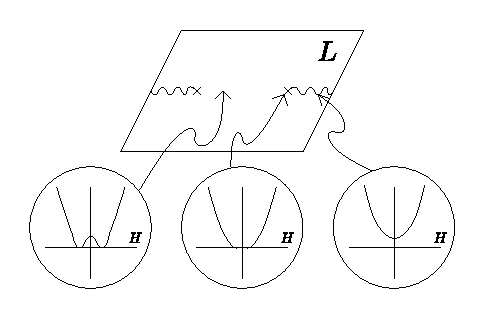
\includegraphics[width=.6\linewidth]{img/effective_potential_branch_cuts.pdf}
	\caption[Behavior of the effective potential $\mcal{W}\[L\]$ in the $L$ plane]{%
		Behavior of the effective potential $\mcal{W}[L]$ in the $L$ plane, based on \cite{Argyres:1996abc}. 
		
		The bubbles illustrate the behavior of the scalar potential $V[H] = \norm{\pd_H \mcal{W}\mspace{1.5mu}[L,H]}^2$ at given values of $\vev{L}$. Note that the vertical axis is not at $H = 0$ but at $H = -m/g$, and the plot covers only $\mbb{R}$eal values of $H$. 
		
		The original illustration in \cite{Argyres:1996abc} seems to be inaccurate. Here we try to clear up the confusions by redrawing parts of the diagrams. 
	}
	\label{fig:effective_potential_branch_cuts}
	\end{figure}
	
	The resulting $\mcal{W}[L]$ have branch points at:
	\begin{equation}
		L = \pm \sqrt{\frac{m^2}{2\lambda g}}\,,
	\end{equation}
	as depicted in \autoref{fig:effective_potential_branch_cuts}. 
	At these points $H$ becomes massless, therefore we should not integrate it out in the first place. Generally, the \textit{effective} mass of $H$ is not simply $m$, but:
	\begin{equation}
		\pd^2_H \mcal{W} \mspace{1.5mu}[L,H]
		\,\big|_{\vev{L},\vev{H}}
		= \pm m \sqrt{
			1 - \vev{L}^2 \Big/ \frac{m^2}{2\lambda g}
		}
	\label{eq:effective_mass}
	\end{equation}
	The 2 signs correspond to the 2 solutions of $\pd_H \mcal{W} = 0$, namely:
	\begin{equation}
		\vev{H}
		= \frac{m}{g} \pqty{
			-1 \pm \sqrt{
				1 - \vev{L}^2 \Big/ \frac{m^2}{2\lambda g}
			}
		\,}
	\label{eq:vev_H}
	\end{equation}
	
%\pagebreak[3]
	
	On the other hand, we can look at the scalar potential:
	\begin{equation}
		V_{\vev{L}} [H] = \norm\big{\,
			\pd_H \mcal{W}\mspace{1.5mu}[L,H]
		\,}^2_{L = \vev{L}}
	\end{equation}
	at \textit{given} values of $\vev{L}$, as shown in \autoref{fig:effective_potential_branch_cuts}. 
	\begin{itemize}
	\item For $
			-\sqrt{\frac{m^2}{2\lambda g}}
			< \vev{L} <
			+\sqrt{\frac{m^2}{2\lambda g}}
		$ there are 2 inequivalent vacua, corresponding to the 2 branches of the square root in \eqref{eq:effective_mass} and \eqref{eq:vev_H}. They are reflected in the low energy effective potential $\mcal{W}[L]$ by the same multi-valued square root structure. 
	
	\item For $\vev{L} = \pm \sqrt{\frac{m^2}{2\lambda g}}$ there is an unique vacuum. This is the branch point in \eqref{eq:effective_mass}, \eqref{eq:vev_H} and $\mcal{W}[L]$. 
	
	\item For $\vev{L} > +\sqrt{\frac{m^2}{2\lambda g}}$ or $\vev{L} < +\sqrt{\frac{m^2}{2\lambda g}}$ it would appear that $V_{\vev{L}} [H] > 0$, and one would suppose that SUSY is spontaneously broken. However, if we allow for $H \in \mbb{C}$, then $V_{\vev{L}} [H] = 0$ can actually be solved with $H \in \mbb{C}$. There are still 2 inequivalent vacua. 
	
	Same applies for generic values of $\vev{L} \in \mbb{C}$. 
	
	\end{itemize}
	
	
\section{SUSY Breaking}
	\speaker{Xia ``Summer'' Gu}\\
	\references{%
%	\begin{enumerate}[noitemsep,topsep=0pt]
%	\item
	\textcite{Argyres:1996abc}, \S9
%	\end{enumerate}
	}\vspace{.5\baselineskip}
	
\section{Super Gauge Theory}
	\speaker{Yihua ``Louiva'' Liu}\\
	\references{%
%	\begin{enumerate}[noitemsep,topsep=0pt]
%	\item
	\textcite{Argyres:1996abc}, \S10
%	\end{enumerate}
	}\vspace{.5\baselineskip}
	
\vspace{1.2\baselineskip}
\pagebreak[4]
\raggedright
\printbibliography[%
%	title = {参考文献} %
	,heading = bibintoc
]
\end{document}
